% MSc thesis style for TU Delft Embedded Networked Systems Group.

% MIT License
%
% Copyright (c) 2023 TU Delft Embedded Systems Group and Casper Dennis van Wezel.
%
% Permission is hereby granted, free of charge, to any person obtaining a copy
% of this software and associated documentation files (the "Software"), to deal
% in the Software without restriction, including without limitation the rights
% to use, copy, modify, merge, publish, distribute, sublicense, and/or sell
% copies of the Software, and to permit persons to whom the Software is
% furnished to do so, subject to the following conditions:
%
% The above copyright notice and this permission notice shall be included in all
% copies or substantial portions of the Software.
%
% THE SOFTWARE IS PROVIDED "AS IS", WITHOUT WARRANTY OF ANY KIND, EXPRESS OR
% IMPLIED, INCLUDING BUT NOT LIMITED TO THE WARRANTIES OF MERCHANTABILITY,
% FITNESS FOR A PARTICULAR PURPOSE AND NONINFRINGEMENT. IN NO EVENT SHALL THE
% AUTHORS OR COPYRIGHT HOLDERS BE LIABLE FOR ANY CLAIM, DAMAGES OR OTHER
% LIABILITY, WHETHER IN AN ACTION OF CONTRACT, TORT OR OTHERWISE, ARISING FROM,
% OUT OF OR IN CONNECTION WITH THE SOFTWARE OR THE USE OR OTHER DEALINGS IN THE
% SOFTWARE.

\documentclass[10pt,twoside,a4paper,openright]{report}

% add new packages here
\usepackage{xcolor}
\usepackage{array}
\usepackage{enumitem}
\usepackage{booktabs}
\usepackage{graphicx}
\usepackage{subcaption}
\usepackage{multirow}
\usepackage[table]{xcolor}
\usepackage[linesnumbered,ruled,vlined]{algorithm2e}
% math packages
\usepackage{amsmath}
\usepackage{amssymb}

% textblocks for title page
\usepackage[absolute]{textpos}

% use babel for proper hyphenation
\usepackage[british]{babel}

% Graphics: different for pdflatex or dvi output, choose one
%%\usepackage[dvips]{graphicx}
%%\usepackage[pdftex]{graphicx}
\usepackage{graphicx}

\usepackage{epstopdf}
\usepackage{rotating}
% \usepackage{subfigure}

% Make captions distinguishable
\usepackage[textfont=bf]{caption}

% Chose font style
\usepackage[scaled=.92]{helvet}

% for url's use "\url{http://www.google.com/}"
\usepackage{url}
\usepackage[plainpages=false]{hyperref} 

% Information that will be filled in at various points in the report
\newcommand{\reportTitle}{Communication-Efficient Splitting Inference in Networked MCUs}
\newcommand{\reportAuthor}{Qi Hong} % Please put your full and official name here: no abbreviations (and to Dutch students: geen roepnamen)
\newcommand{\studentNumber}{6125166}
\newcommand{\reportEmailTUD}{qihong@tudelft.nl}
\newcommand{\reportEmailNonTUD}{qhong0912@gmail.com}
\newcommand{\reportUrlEmailTUD}{\href{mailto:\reportEmailTUD}{\reportEmailTUD}}
\newcommand{\reportUrlEmailNonTUD}{\href{mailto:\reportEmailNonTUD}{\reportEmailNonTUD}}
\newcommand{\reportMSC}{Computer \& Embedded Systems Engineering} % Examples are {Embedded Systems} {Computer Engineering} {Computer Science} or {Electrical Engineering}
\newcommand{\reportDate}{July 7, 2026}
\newcommand{\presentationDate}{July 14, 2026}
\newcommand{\graduationCommittee}{
prof. Qing Wang & Delft University of Technology \\
prof. Jie Yang & Delft University of Technology \\
% ...
}

% Provide full name and surname (no abbreviations), so "Koen Langendoen" not "K. Langendoen"

% The order of listing above: 

% title + Graduation committee chairman name and surname (chairman)
% title + Supervisor 1 name and surname (direct supervisor)
% title + Supervisor 2 name and surname (direct supervisor)
% ...
% title + Supervisor X name and surname (direct supervisor) 
% ...
% Others (ordered by title and alphabetical)

% Example: 
% prof.\,dr.\,Koen Langendoen (chairman) & Delft University of Technology \\ 
% dr.\,Przemys{\l}aw Pawe{\l}czak & Delft University of Technology \\ 

\newcommand{\reportAbstract}{
The Tiny Machine Learning (TinyML) brings deep learning to microcontrollers (MCUs), but the few hundred kilobytes of SRAM available on these devices make deployment difficult. While model weights can reside in Flash, the intermediate activations generated at inference must fit in SRAM. For the efficient convolutional neural networks (CNNs) that dominate TinyML, such as MobileNetV2, MCUNet, MnasNet, and ProxylessNAS, it is the peak activation footprint rather than the model size that limits deployment. Because these networks are built from Inverted Residual Blocks (IRBs), whose expand–depthwise–project structure produces a large temporary activation inside each block that can exceed the SRAM of a single MCU.
Distributing CNNs across several networked MCUs can aggregate their memory, but existing distributed runtimes communicate at layer or sub-layer boundaries. This turns the expanded activation inside each IRB into a network-level object that must traverse the network twice and be buffered in full at the coordinating device, creating a both communication and memory bottleneck.

This thesis presents a framework that transforms a standard CNN into a communication-efficient distributed execution across a cluster of networked MCUs. An offline stage quantizes the model to INT8 and compiles it into a communication-aware execution plan and per-worker manifests. An online stage executes the plan on a coordinator–worker cluster. There are two novel mechanisms in the system: \emph{block-wise local execution}, which keeps each expanded activation inside a worker, and \emph{cross-block data reuse}, which exchanges only the thin boundary rows between consecutive blocks. 
% An overlap-ratio cost model is proposed to characterize when block-wise execution stops paying off and enables an adaptive per-block choice.

We implement the framework on a network of six MCUs and evaluate it on four representative IRB-based CNNs. Compared with naive layer-wise execution, our framework reduces early-block communication overhead by over 80\%, latency by up to 47\%, and coordinator peak SRAM from 735 KB to 158 KB.
}

\newcommand{\reportKeywords}{TinyML, Split Inference, Edge Computing}

% Did the thesis lead to a paper? 
% e.g. The work presented in this thesis has lead to a paper which has been submitted to a conference for publication, pending peer-review
%\newcommand{\reportPaper}{LINE ABOUT YOUR PUBLICATION GOES HERE}
\newcommand{\reportPaper}{The work presented in this thesis has lead to a paper which has been submitted to a conference for publication, pending peer-review.}


% Information for pdflatex
\pdfinfo{
/Author (\reportAuthor)
/Title (\reportTitle)
/Keywords (\reportKeywords)
}

\begin{document}

\pagenumbering{alph}
\pagestyle{empty}

% Make frontcover
\input{template/frontcover}

% Set marginns
\hoffset=1.63cm
\oddsidemargin=0in
\evensidemargin=0in
\textwidth=5in

%
\parindent=1em

% Empty page
\cleardoublepage

\pagestyle{plain}
\pagenumbering{roman}
\setcounter{page}{1}

% Create title page: page i (hidden)
\input{template/titlepage}

% Create Graduation Data and Abstract: pages ii and iii (hidden)
\input{template/graduationdata}

% Empty page: page iv
\cleardoublepage

% (Optional) Include quotation: page v (uncomment if needed)
\thispagestyle{empty}

\null\vfill

\begin{center}
\emph{``So we beat on, boats against the current, borne back ceaselessly into the past.''} -- F. Scott Fitzgerald
\end{center}

\vspace{10cm}

\clearpage


% Empty page: page vi
\cleardoublepage

% Create preface: page v
\chapter*{Preface}
\addcontentsline{toc}{chapter}{Preface}

% Put a motivation for a research topic here.

This thesis builds upon the previous master's thesis, ``Split CNN Inference on Networked Microcontrollers", by Junyu Lu. Deploying deep learning inference on edge devices has become an increasingly important research direction in recent years, particularly with the rapid advancement of Large Language Models (LLMs). While distributed inference enables resource-constrained devices to execute complex neural networks collaboratively, it also introduces communication overhead as a major performance bottleneck. Therefore, the primary objective of this research is to investigate communication-efficient distributed inference systems that can be deployed on Microcontroller Units (MCUs). In this thesis, we focus on convolutional neural networks (CNNs) as the first step toward this goal. Extending these techniques to transformer-based models remains an important direction for future research.

During the nearly nine months of my master's thesis, I gained valuable research experience and learned a great deal about both embedded AI systems and academic research. I sincerely hope that the findings presented in this thesis will be helpful to future researchers who are interested in this field and contribute to the continued development of communication-efficient distributed inference on resource-constrained devices. 

This work would not have been possible without the support of many people. First and foremost, I would like to express my sincere gratitude to my supervisor, Prof. Qing Wang, for his invaluable guidance, encouragement, and continuous support throughout this thesis. I am deeply grateful to Ph.D. candidate Hao Liu for his patience, insightful discussions, and generous assistance during my research. I also want to thank Prof. Jie Yang for being a committee member of my thesis defense. I would also like to acknowledge ChatGPT and Claude, which have become valuable research assistants in the era of generative AI. They greatly improved my productivity by helping me explore ideas, debug code, and polish academic writing. My sincere thanks also go to all my friends in the Netherlands for their encouragement, companionship, and support throughout my studies. Finally, and most importantly, I would like to thank my family for their unconditional love, understanding, and unwavering encouragement. Without their continuous support, I would not have been able to complete this journey. 

To everyone who has supported me along the way, thank you.



% This research is the following research after a Master thesis ``Split CNN Inference on Networked Microcontrollers" from Junyu Lu. Deploying inference in the edge device is a more and more popular trend during these years, especially after the LLM emerges. Distributed inference introduces the potential communication bottleneck in the previous research. So how to design a communication-efficient system deployable in MCUs is our main research topic. The CNNs are the firt step. How to deploy the transformer-based models is also an important extensions in the future work.

% During nearly nine months of my master thesis, I gained many insights. And I truly wish it could help others who still want to contribute to this research area.

% I could not have finished this work without a series of support. First and foremost, I want to express my grateful thanks to my supervisor Prof. Qing Wang, and Ph.D candidate Hao Liu for their patience and brilliant guidance. I also want to thanks to ChatGPT and Claude especially in this AI era. I also want to thanks all my friends in Delft who support me a lot during the study. Last but not least, I want to thank my family. Without their support and encouragement, I could not finish the study. Thanks for all of your guys.  


\vspace{1\baselineskip}

\reportAuthor

\vspace{1\baselineskip}

\noindent
Delft, The Netherlands

\noindent
\today

% Empty page: page vi
\cleardoublepage

% Create tabe of contents: page vii
\tableofcontents

\cleardoublepage

\pagenumbering{arabic}
\setcounter{page}{1}

% Create Introduction: page 1
% \chapter{Introduction}
\label{chp:introduction}

Introduction goes here. Introduction goes here.Introduction goes here.Introduction goes here.Introduction goes here.Introduction goes here.Introduction goes here.Introduction goes here.Introduction goes here.Introduction goes here.Introduction goes here.Introduction goes here.Introduction goes here.Introduction goes here.Introduction goes here.Introduction goes here.Introduction goes here.Introduction goes here.Introduction goes here.Introduction goes here.Introduction goes here.Introduction goes here.Introduction goes here.Introduction goes here.Introduction goes here.Introduction goes here.Introduction goes here.Introduction goes here.Introduction goes here.Introduction goes here.Introduction goes here.Introduction goes here.Introduction goes here.Introduction goes here.Introduction goes here.Introduction goes here.Introduction goes here.Introduction goes here.Introduction goes here.Introduction goes here.Introduction goes here.Introduction goes here.Introduction goes here.Introduction goes here.Introduction goes here.Introduction goes here.Introduction goes here.Introduction goes here.Introduction goes here.Introduction goes here.Introduction goes here.

% Create chapters
\chapter{Introduction}
\label{chp:introduction}

Introduction goes here. Introduction goes here.Introduction goes here.Introduction goes here.Introduction goes here.Introduction goes here.Introduction goes here.Introduction goes here.Introduction goes here.Introduction goes here.Introduction goes here.Introduction goes here.Introduction goes here.Introduction goes here.Introduction goes here.Introduction goes here.Introduction goes here.Introduction goes here.Introduction goes here.Introduction goes here.Introduction goes here.Introduction goes here.Introduction goes here.Introduction goes here.Introduction goes here.Introduction goes here.Introduction goes here.Introduction goes here.Introduction goes here.Introduction goes here.Introduction goes here.Introduction goes here.Introduction goes here.Introduction goes here.Introduction goes here.Introduction goes here.Introduction goes here.Introduction goes here.Introduction goes here.Introduction goes here.Introduction goes here.Introduction goes here.Introduction goes here.Introduction goes here.Introduction goes here.Introduction goes here.Introduction goes here.Introduction goes here.Introduction goes here.Introduction goes here.Introduction goes here.
\chapter{Related Work}
\label{chp:related-work}

Related work
\chapter{System Design}
\label{chp:system_design}
% In this section, we will present the design of our framework that transforms a standard single-device CNN into a communication-efficient distributed execution tasks across a cluster of networked MCUs. We will first discuss the overall architecture of coordinator-worker model, followed by the communication protocols. Two core optimizations techniques, i.e., \emph{block-wise local execution} and \emph{cross-block data reuse}, are proposed to allieviate the communication overhead, and will be discussed in detail. \textcolor{red}{We analyze the conditions for our proposed optimizations.} 
%% and provide a cost model to evaluate the trade-offs between communication and computation. Finally, we will discuss the implementation details of our framework.

In this chapter, we present the design of our framework that transforms a standard single-device CNN into a set of communication-efficient distributed execution tasks across a cluster of networked MCUs. We first describe the overall coordinator-worker architecture and a two-stage execution pipeline. Then, we detail the offline preprocessing stage, which quantizes the CNN model and compiles it into an execution plan in JSON format (Section~\ref{sec:offline-preprocessing}), and the online inference stage, which carries out the plan over a lightweight application protocol in TCP/IP (Section~\ref{sec:online-inference}). On top of this runtime inference, we develop two core optimization techniques that alleviate the communication and memory overhead of the system: \emph{block-wise local execution} (Section~\ref{sec:block-wise-local-execution}) and \emph{cross-block data reuse} (Section~\ref{sec:cross-block-data-reuse}). Between these two optimizations, we introduce an \emph{overlap-ratio cost model} (Section~\ref{sec:overlap-ratio-cost-model}) that characterizes when block-wise local execution stops paying off, and for cross-block data reuse we analyze the conditions under which it preserves correctness and improves performance (Section~\ref{sec:cross-conditions}). 

\section{System Architecture}
\label{sec:system-architecture}

\begin{figure}[t]
    \center
    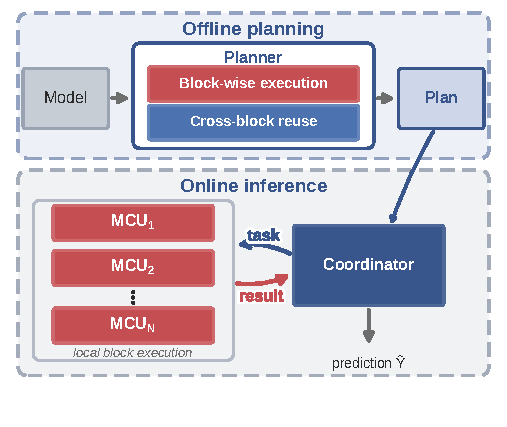
\includegraphics[width=\textwidth,height=0.3\textheight,keepaspectratio]{figs/fig_overview.pdf}
    \caption{Overview of our system architecture, comprising an offline preprocessing stage that compiles the model into an execution plan and per-worker manifests, and an online stage that executes the plan on a coordinator-worker cluster.}
    % \vspace{-4mm}
    \label{fig:system-architecture}
\end{figure}

As discussed in Section~\ref{chp:system_design}, a typical MCU offers only hundreds of KBs of SRAM (e.g., less than 512~KB) during runtime inference. \textcolor{red}{While the model weights can be stored in Flash memory, the intermediate activations must reside in SRAM at runtime. For CNNs built from IRBs, the largest tensor at runtime is the output of the expanding convolution layer: each block first expands the channel dimension by an expansion ratio $e$ (e.g., $e=6$ in MobileNetV2), applies a depthwise convolution, and then reduces the channel dimension back to the original size (refs).} The output of the expanding convolution layer is therefore $e$ times larger than the input, which can easily exceed the SRAM capacity of a single MCU. This results in a significant memory bottleneck that prevents the execution of large CNNs on resource-constrained MCUs. 

To address this, we implement an end-to-end pipeline for distributed inference across multiple networked MCUs, as shown in Figure~\ref{fig:system-architecture}, comprising two stages:
\begin{itemize}
    \item \textbf{Offline preprocessing stage}: It performs an 8-bit quantization of the model, and extracts the metadata describing the model weights and structural information. The metadata is emitted as JSON files and serialized into the Flash memory of each MCU at compilation time. An \emph{execution plan} is generated that describes the inference strategy and the data flow between the MCUs.
    
    \item \textbf{Online inference stage}: It executes the model on the distributed system across multiple networked MCUs. A single \emph{coordinator} holds the model metadata and the execution plan, partitions the workload to the \emph{workers} at each step, and reassembles the workers' outputs to produce the final inference result. Each \emph{worker} stores its share of the weights and activations, and performs the assigned computation tasks. The coordinator and workers communicate through a lightweight protocol on top of TCP/IP.
\end{itemize}

% As discussed in Section~\ref{chp:system_design}, a typical MCU offers only hundreds of KBs of SRAM (e.g., less than 512~KB) during runtime inference. While the model weights could be stored in the Flash memory, the intermediate activations have to reside in the SRAM at runtime, resulting in a significant memory bottleneck. 

% To address the issue, we implement a end-to-end pipeline shown in Figure~\ref{fig:tbd} that incorporates:
% \begin{itemize}
%     \item \textbf{Offline preprocessing stage} that quantizes the model, and extracts the metadata for the model weights and intermediate activations. The metadata will be released as JSON files and serialized into the Flash memory of each MCU at compilation time. An \emph{execution plan} will be generated to describe inference strategy and the data flow between the MCUs. 
    
%     \item \textbf{Online inference stage} that executes the model in the distributed system across multiple networked MCUs. A single \emph{coordinator} holds the model metadata and the execution plan, partitions the workload to the \emph{workers} at each step, and reassables the workers' outputs to produce the final inference result. Each \emph{worker} stores its share of the weights and activations and performs the assigned computation tasks. The coordinator and workers communicate through a lightweight protocol under TCP/IP. 
% \end{itemize}

\section{Offline Preprocessing}
\label{sec:offline-preprocessing}


\subsection{Quantization}

\subsection{Planner}


\section{Online Inference}
\label{sec:online-inference}
The coordinator-worker architecture is designed to execute the distributed inference tasks efficiently. As demonstrated in Figure~\ref{fig:tbd}, a coordinator is responsbile for the task scheduling and data aggregation. Based on the execution plan, the coordinator partitions the input activations, wraps and assigns the computation tasks to workers, and gather results from workers to produce the output activations. Each worker is in charge of executing the assigned tasks, which includes loading model weights in Flash, selecting the suitable computation kernel, and performing the computation on the input activations.

\subsection{Coordinator Design}

\subsection{Worker Design}

\subsection{Protocol Design}




\section{Block-wise Local Execution}
\label{sec:block-wise-local-execution}
To optimize performance and resource utilization, we have implemented a block-wise local execution strategy. This approach allows us to process data in smaller chunks, reducing memory overhead and improving execution speed. Each block is processed independently, allowing for parallel execution and better load balancing across the system. This design choice also enhances fault tolerance, as failures in one block do not affect the processing of others.

\section{Overlap-ratio Cost Model}
\label{sec:overlap-ratio-cost-model}
We have implemented a hybrid scheduling mechanism that combines the benefits of both centralized and decentralized approaches. This allows for more efficient resource allocation and load balancing across the system.

\section{Cross-block Data Reuse}
\label{sec:cross-block-data-reuse}
To further optimize performance, we have implemented a cross-block data reuse mechanism. This allows data generated in one block to be efficiently utilized in subsequent blocks, reducing redundant computations and improving overall system efficiency.

\section{Conditions to Enable Cross-block Data Reuse}
\label{sec:cross-conditions}
Some conditions for cross-block data reuse include:
\begin{itemize}
    \item Data must be compatible across blocks.
    \item The data must be stored in a format that allows for easy retrieval and reuse.
    \item The system must ensure that the reused data is up-to-date and valid for the current block's processing requirements.
\end{itemize}





\chapter{Implementation}
\label{chp:implementation}

\textcolor{red}{Need to rephrase}
This chapter describes the implementation of the system design presented in Chapter~\ref{chp:system_design} on real hardware. The framework consists of two codebases. A Python codebase that implements the preprocessing toolchains and evaluation scripts, and a real deployment codebase that realizes an asynchrnous Python coordinator with a cluster of Teensy 4.1 workers written in C++. We first describe the hardware platform employed in the experiments in Section~\ref{sec:implementation-hardware-platform}. Section~\ref{sec:offline-preprocessing} describes the offline toolchains that compile a pretained model into manifests and firmware. Section~\ref{sec:implementation-worker-runtime} to section\ref{sec:implementation-communication-protocol} describe the runtime implementations of the coordinator and workers on the MCU. We further explains how we validate the numerical correctness of the system in Section~\ref{sec:implementation-validation}. Finally, we discuss some engineering details in Section~\ref{sec:implementation-miscellaneous}.


\section{Hardware Platform}
\label{sec:implementation-hardware-platform}
Teensy 4.1 board is employed as the worker in our experiments. It is built with an NXP i.MX RT1062 microcontroller. The device has an Arm Cortex-M7 core running at 600 MHz with a hardware floating-point unit. The board has two 512 KB RAM and 8 MB Flash memory without a memory management unit. Network support is provided by an external Ethernet PHY chip with NativeEthernet library. The testbed connects up to six boards to a single TP-Link TL-SG116 gigabit switch. To simplify profiling and data collection, a Linux PC servers as the coordinator, while the worker-side execution runs on MCUs.

\section{Offline Toochain}
\label{sec:implementation-offline-toolchain}
















\section{Coordinator Runtime}
\label{sec:implementation-coordinator-runtime}

\section{Worker Runtime}
\label{sec:implementation-worker-runtime}

\section{Communication Protocol}
\label{sec:implementation-communication-protocol}


\section{Validation}
\label{sec:implementation-validation}

\section{Miscellaneous}
\label{sec:implementation-miscellaneous}


\chapter{Evaluation}
\label{chp:evaluation}
In this section, we evaluate the performance of our framework on real hardware. Section~\ref{sec:eval-exp-setup} first presents the experimental setup in detail. We first evaluate how much does our framework reduce the communication overhead in Section~\ref{sec:eval-comm-overhead}. Then we evaluate the end-to-end inference latency in Section~\ref{sec:eval-end2end-infer-latency}. Finally, we evaluate the peak memory usage of our framework in Section~\ref{sec:eval-peak-memory} and conduct an ablation study in Section~\ref{sec:eval-ablation-study}.



\section{Experiment Setup}
\label{sec:eval-exp-setup}

% \begin{table}[t]
%     \centering
%     \caption{Evaluated models. All are built from inverted residual blocks and
%     quantised to INT8. The last column is the peak activation footprint a single MCU would need, which exceeds the SRAM of a Teensy 4.1 in every case.}
%     \label{tab:eval-models}
%     \begin{tabular}{l c c c c}
%         \hline
%         \textbf{Model} & \textbf{Input} & \textbf{Expansion} & \textbf{DW kernel} &
%         \textbf{Peak mem.} \\
%         \hline
%         MobileNetV2-0.35 & $224^2$ & 6 & 3 & 735~KB \\
%         MnasNet-0.5 & $224^2$ & 3 to 6 & 3, 5 & 392~KB \\
%         MCUNet-in4 & $160^2$ & 3 to 5 & 3, 5, 7 & 400~KB \\
%         ProxylessNAS & $224^2$ & 3 to 6 & 3, 5, 7 & 784~KB \\
%         \hline
%     \end{tabular}
% \end{table}





% We evaluate our system on a testbed consisting of up to 8 Teensy 4.1 as workers with four representative CNNs for edge vision tasks. 
\subsection{Hardware}
As described in Section~\ref{sec:implementation-hardware-platform}, the testbed consists of up to 8 Teensy 4.1 boards as workers and a TP-Link TL-SG116 gigabit switch to connect the workers and the coordinator. 

\subsection{Models}
\begin{table}[b]
    \caption{Evaluated models. All weights and activations are quantized to INT8 and stored in Flash and SRAM.}
    \label{tab:eval-models}
    \centering
    \setlength{\tabcolsep}{8pt}
    \resizebox{\columnwidth}{!}{%
    \begin{tabular}{c c c c c}
        \toprule
        \textbf{Model} & \textbf{Input} & \textbf{Expansion} & \textbf{DW Kernel} & \textbf{Peak Mem.} \\
        \midrule
        MobileNetV2-0.35 & $224^2$ & $6$      & $3$     & $735$\,KB \\
        MnasNet-0.5      & $224^2$ & $3$--$6$ & $3,5$   & $392$\,KB \\
        MCUNet-in4       & $160^2$ & $3$--$5$ & $3,5,7$ & $400$\,KB \\
        ProxylessNAS     & $224^2$ & $3$--$6$ & $3,5,7$ & $784$\,KB \\
        \bottomrule
    \end{tabular}}
\end{table}

We evaluate four representative CNNs for edge vision tasks listed in Table~\ref{tab:eval-models}. All these four models are built from inverted residual blocks, a common design for efficient CNNs, with different expansion ratios and depthwise kernel sizes. Every model is quantized to INT8 by the offline preprocessing. The last peak memory in Table~\ref{tab:eval-models} is the peak activation footprint if only a single MCU is used during inference.

\subsection{Baseline and metrics}
We compare our framework with a baseline that runs the same models in a naive layer-wise strategy which communicates at every layer boundary and holds each intermediate feature map in full at the coordinator. Our framework adds the two core mechanisms (\emph{A: block-wise local execution} and \emph{B: cross-block data reuse}) to the baseline as discussed in Section~\ref{sec:block-wise-local-execution} and Section~\ref{sec:cross-block-data-reuse}.

We evaluate from three aspects: communication overhead, end-to-end inference latency, and peak memory footprint. Communication overhead measures the total amount of data transferred between the coordinator and workers during inference. End-to-end inference latency measures the time taken from sending the input to receiving the output. Peak memory footprint measures the maximum memory used by the coordinator and workers at runtime, as memory is a critical resource on MCUs.

\section{Communication Overhead}
\label{sec:eval-comm-overhead}
We first break down inference to isolate the communication cost. Figure~\ref{fig:tbd} reports the communication latency of the initial convolution and the first four inverted residual blocks on four workers for each model. These early layers operate on the largeset feature maps and therefore expose the communication cost most clearly.

The communication overhead dominates these layers in the baseline system. The communication latency of the first IRB reaches about 39 ms on MobileNetV2-0.35, 74 ms on MnasNet-0.5, 79 ms on MCUNet-in4, and 156 ms on ProxylessNAS. Since the output of each layer needs to be sent to the coordinator and then re-scattered to the workers, the network transfer of intermediate activations becomes a significant bottleneck. 

\emph{Ours} significantly reduces the communication overhead. Our block-wise local execution keeps the expanded activation inside the worker so that it never needs to cross the network. Our cross-block data reuse only requires the communication of the thin boundary rows between adjacent workers. Therefore, the per-block communication latency falls to a few milliseconds. On the first IRB of ProxylessNAS, the latency reduction is approximately 94\%. \emph{Ours} consistently outperforms the baseline across all models and layers, demonstrating the effectiveness of our framework in reducing communication overhead.




































\section{End-to-end Inference Latency}
\label{sec:eval-end2end-infer-latency}


\section{Peak Memory}
\label{sec:eval-peak-memory}

\section{Ablation Study}
\label{sec:eval-ablation-study}
\chapter{Conclusions and Future Work}
\label{chp:conclusions}

Conculsions.


\section{Conclusion}


\section{Limitations and future work}


% Create bibliography
\bibliographystyle{plain} % Please do not change the style of bibliography (yes, it should be `plain`)
\bibliography{bib/MyMScTUDESThesisBibFile} % remove "../" before "bib" if you compile directly in Overleaf or in your favourite local LaTeX distribution

% Create appendix
\appendix
\chapter{Experiments across six MCUs}
\label{app:appendix_a}

% Appendix body.
This appendix presents the complete per-block profiling results for all evaluated configurations with two to six MCUs, complementing the summary results presented in Chapter~\ref{chp:evaluation}.

Figure~\ref{fig:results-comm-appendix} presents the complete communication overhead for configurations ranging from two to six MCUs. Figure~\ref{fig:results-memory-appendix} shows the coordinator's peak memory usage across the same range of worker counts, while Figure~\ref{fig:results-memory-worker-appendix} reports the corresponding peak memory usage of the worker MCUs.

In each figure, subfigures~(a)--(d) correspond to the four representative models evaluated in this thesis. \emph{Baseline} denotes layer-wise execution without activation reuse, whereas \emph{Ours} denotes block-wise local execution with cross-block data reuse.


\begin{figure}[t]
    \centering
        % MobileNetV2-0.35
      \begin{subfigure}{0.24\linewidth}
        \centering
        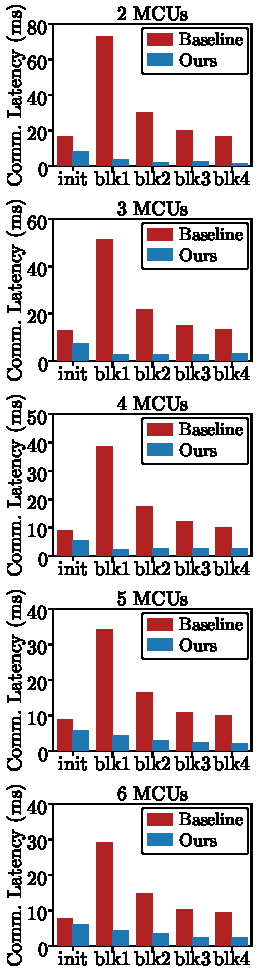
\includegraphics[width=\linewidth]{figs/comm/appendix/comm_mobilenetv2_035.pdf}
        % \vspace{-2mm}
        \caption{MobileNetV2}
        \label{fig:comm-mbv2-appendix}
      \end{subfigure}
      % \hspace{1mm}
        % MCUNet
      \begin{subfigure}{0.24\linewidth}
        \centering
        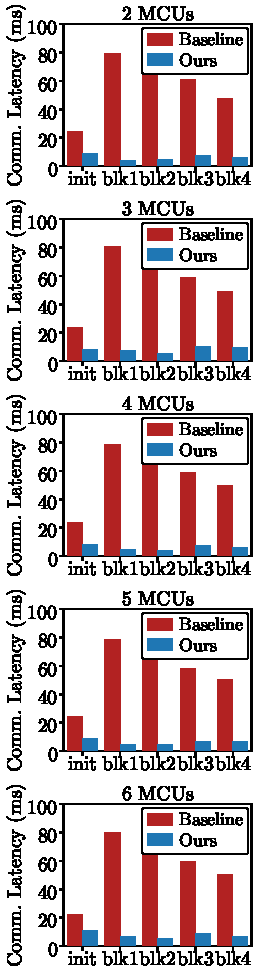
\includegraphics[width=\linewidth]{figs/comm/appendix/comm_mcunet.pdf}
        % \vspace{-2mm}
        \caption{MCUNet}
        \label{fig:comm-mcunet-appendix}
      \end{subfigure}
      % \\ \vspace{1mm}
      \begin{subfigure}{0.24\linewidth}
        \centering
        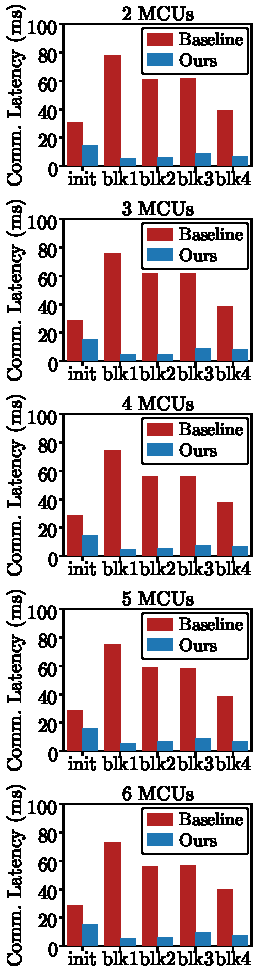
\includegraphics[width=\linewidth]{figs/comm/appendix/comm_mnasnet_05.pdf}
        % \vspace{-2mm}
        \caption{MnasNet-0.5}
        \label{fig:comm-mnasnet-appendix}
      \end{subfigure}
      % \hspace{1mm}
        % ProxylessNAS-Mobile
      \begin{subfigure}{0.24\linewidth}
        \centering
        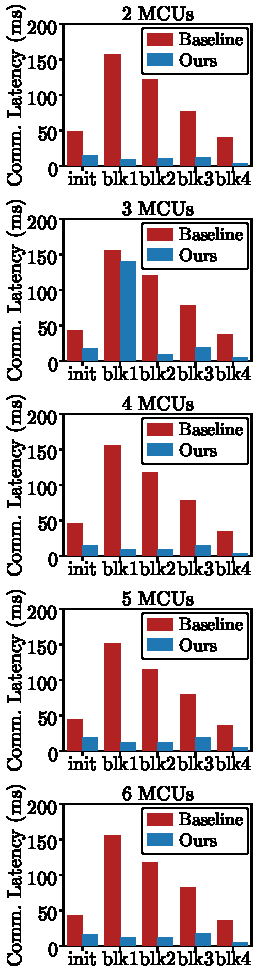
\includegraphics[width=\linewidth]{figs/comm/appendix/comm_proxylessnas_mobile.pdf}
        % \vspace{-2mm}
        \caption{ProxylessNAS}
        \label{fig:comm-proxylessnas-appendix}
      \end{subfigure}
      % \hfill
  \caption{Communication overhead.}
  \label{fig:results-comm-appendix}
\end{figure}



\begin{figure}[t]
    \centering
        % MobileNetV2-0.35
      \begin{subfigure}{0.24\linewidth}
        \centering
        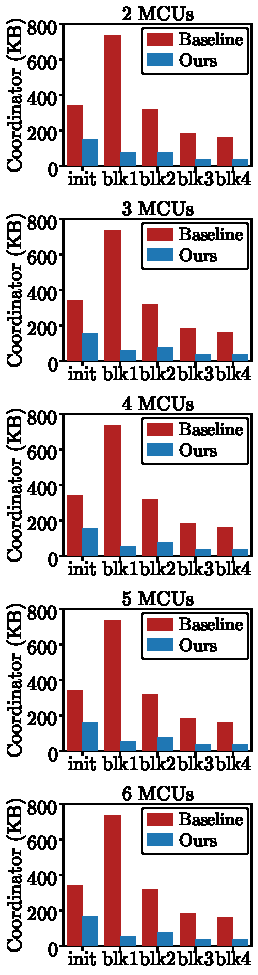
\includegraphics[width=\linewidth]{figs/memory/appendix/coord_mobilenetv2_035.pdf}
        % \vspace{-2mm}
        \caption{MobileNetV2}
        \label{fig:memory-mbv2-appendix}
      \end{subfigure}
      % \hspace{1mm}
        % MCUNet
      \begin{subfigure}{0.24\linewidth}
        \centering
        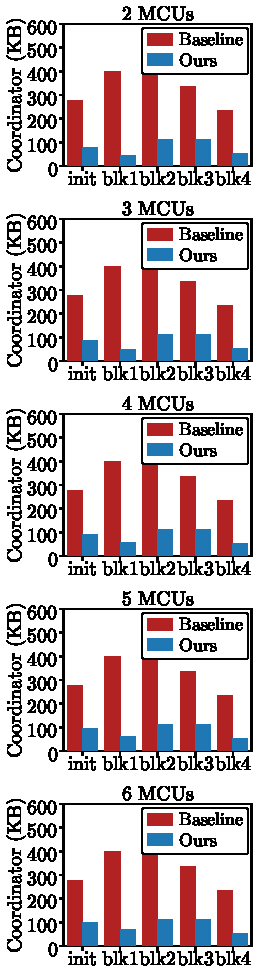
\includegraphics[width=\linewidth]{figs/memory/appendix/coord_mcunet.pdf}
        % \vspace{-2mm}
        \caption{MCUNet}
        \label{fig:memory-mcunet-appendix}
      \end{subfigure}
      % \\ \vspace{1mm}
      \begin{subfigure}{0.24\linewidth}
        \centering
        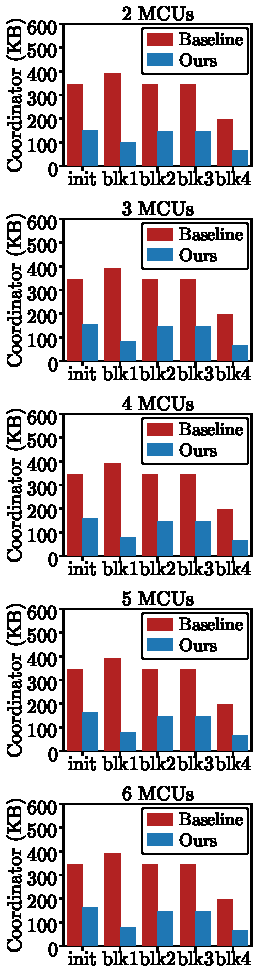
\includegraphics[width=\linewidth]{figs/memory/appendix/coord_mnasnet_05.pdf}
        % \vspace{-2mm}
        \caption{MnasNet-0.5}
        \label{fig:memory-mnasnet-appendix}
      \end{subfigure}
      % \hspace{1mm}
        % ProxylessNAS-Mobile
      \begin{subfigure}{0.24\linewidth}
        \centering
        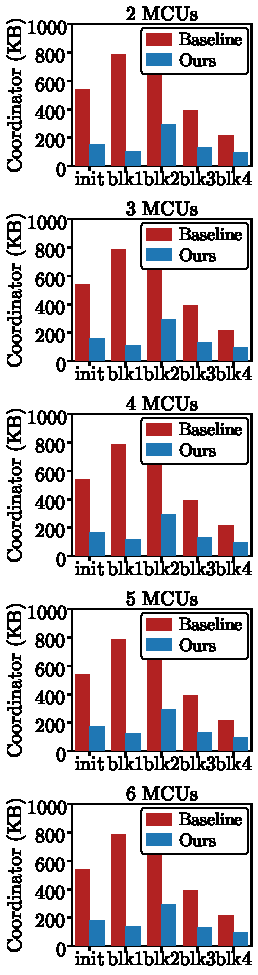
\includegraphics[width=\linewidth]{figs/memory/appendix/coord_proxylessnas_mobile.pdf}
        % \vspace{-2mm}
        \caption{ProxylessNAS}
        \label{fig:memory-proxylessnas-appendix}
      \end{subfigure}
      % \hfill
  \caption{The peak memory usage at the coordinator.}
  \label{fig:results-memory-appendix}
\end{figure}

\begin{figure}[t]
    \centering
        % MobileNetV2-0.35
      \begin{subfigure}{0.24\linewidth}
        \centering
        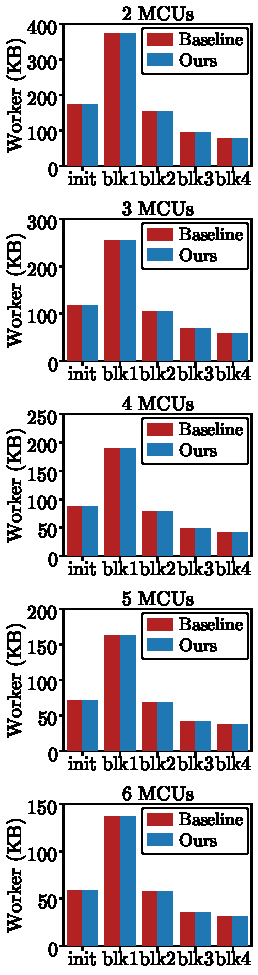
\includegraphics[width=\linewidth]{figs/memory/appendix/worker_mobilenetv2_035.pdf}
        % \vspace{-2mm}
        \caption{MobileNetV2}
        \label{fig:memory-mbv2-worker-appendix}
      \end{subfigure}
      % \hspace{1mm}
        % MCUNet
      \begin{subfigure}{0.24\linewidth}
        \centering
        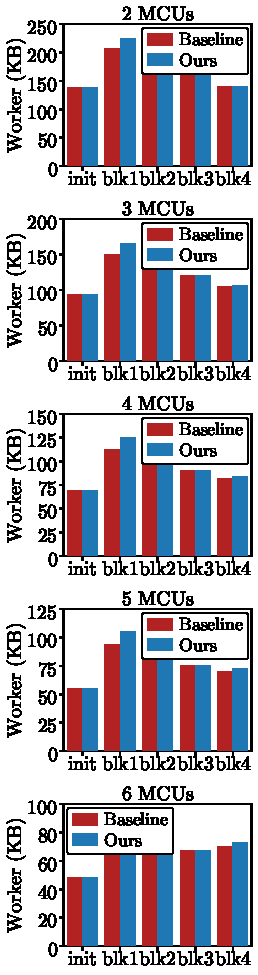
\includegraphics[width=\linewidth]{figs/memory/appendix/worker_mcunet.pdf}
        % \vspace{-2mm}
        \caption{MCUNet}
        \label{fig:memory-mcunet-worker-appendix}
      \end{subfigure}
      % \\ \vspace{1mm}
      \begin{subfigure}{0.24\linewidth}
        \centering
        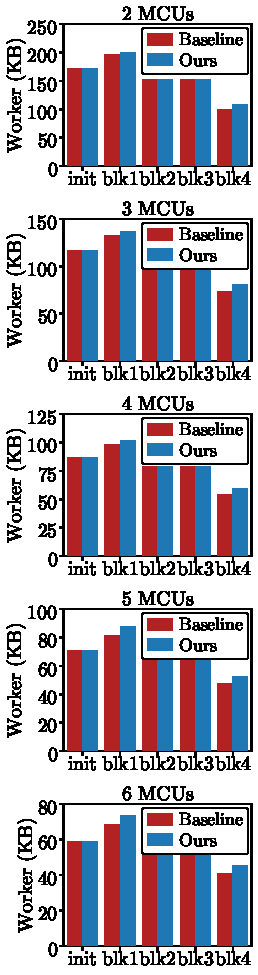
\includegraphics[width=\linewidth]{figs/memory/appendix/worker_mnasnet_05.pdf}
        % \vspace{-2mm}
        \caption{MnasNet-0.5}
        \label{fig:memory-mnasnet-worker-appendix}
      \end{subfigure}
      % \hspace{1mm}
        % ProxylessNAS-Mobile
      \begin{subfigure}{0.24\linewidth}
        \centering
        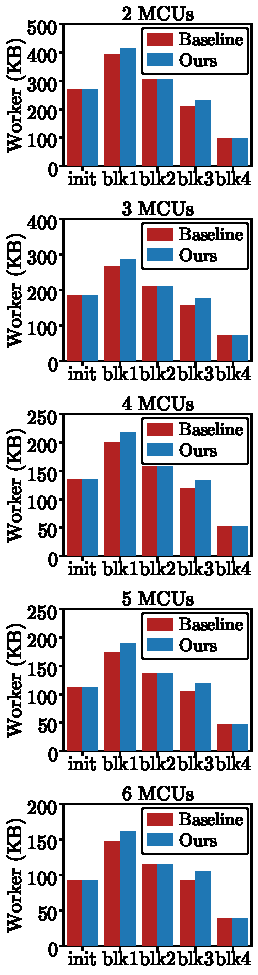
\includegraphics[width=\linewidth]{figs/memory/appendix/worker_proxylessnas_mobile.pdf}
        % \vspace{-2mm}
        \caption{ProxylessNAS}
        \label{fig:memory-proxylessnas-worker-appendix}
      \end{subfigure}
      % \hfill
  \caption{The peak memory usage at the workers.}
  \label{fig:results-memory-worker-appendix}
\end{figure}

\end{document}
